% Létrehozva: 2009. június 28.
\documentclass[12pt,a4paper,twoside]{article}

% Hosszú sorok helyett inkább sok hely szavak között
\sloppy

% Táblázatok formázásához
\usepackage{array}
\usepackage{multirow}

% Ábrák
\usepackage{graphicx}
\usepackage{float}

% Ékezetek, magyar nyelv
\usepackage[utf8]{inputenc}
\usepackage[T1]{fontenc}
\usepackage[hungarian]{babel}

% Forráskód megjelenítésére
\usepackage{listings}
\lstset{
  numbers=left,
  frame=shadowbox,
  numberstyle=\tiny,
  basicstyle=\ttfamily\small
}

% Definíciós lista kis whitespace-el
\newcommand{\desc}{
  \begin{description}{}{}
    \setlength\itemsep{0pt}
    \setlength\parskip{0pt}
    \setlength\topsep{0pt}
    \setlength\partopsep{0pt}
    \small}
  \newcommand{\ed}{
  \end{description}
}

% Itemize környezetbe, fájlok leírására
\newcommand{\fitem}[1]{\item \texttt{#1}:}

% Elemek műveleteinek és tulajdonságainak leírásához
\usepackage{ifthen}
\newcommand{\elem}[3]{
  \vspace{1cm}
  \hspace{-.7cm}
  \begin{tabular*}{\textwidth}{rl}
  \hline
  \multicolumn{2}{c}{\large\texttt{#1}\normalsize}\\
  \hline
  \ifthenelse{\not{\equal{#2}{-}}}{
    \textbf{Műveletek:} & \parbox{9.5cm}{#2}\\\vspace{-.4cm}&
    \ifthenelse{\not{\equal{#3}{-}}}{\\}{}
  }{}
  \ifthenelse{\not{\equal{#3}{-}}}{
    \textbf{Tulajdonságok:} & \parbox{9.5cm}{#3}
    \\
  }{}
  \end{tabular*}

}
% Elvárás a szakdolgozattal szemben a Times - sebaj
%\usepackage{times}
\fontfamily{garamond}

% Az elektronikus változatban hiperhivatkozások
\usepackage{hyperref}
% PDF tulajdonságai
\hypersetup{
  bookmarks=true,
  unicode=true,
  pdftoolbar=true,
  pdfmenubar=true,
  pdffitwindow=false,
  pdfstartview={FitH},
  pdftitle={Szakdolgozat},
  pdfauthor={Nagy Zoltán},
  pdfsubject={Online űrlapkészítő},
  pdfnewwindow=true,
  colorlinks=true
}

% Nyomtatásba
\hypersetup{
  linkcolor=black,
  citecolor=black,
  filecolor=black,
  urlcolor=black
}

% Elektronikus változat
\hypersetup{
  linkcolor=red,
  citecolor=green,
  filecolor=magenta,
  urlcolor=cyan
}

% "Oldalbeállítás"
\usepackage[margin=2.5cm, bmargin=3cm, bindingoffset=2cm]{geometry}

% Fejléc
\usepackage{extramarks}
\usepackage{fancyhdr}
\pagestyle{fancy}
\renewcommand{\sectionmark}[1]{\markright{#1}{}}
\fancyhf{}
\fancyhead[RE,LO]{\thepage}
\fancyhead[RO,LE]{\rightmark}


\title{Szakdolgozat\\\normalsize Online űrlapkészítő}
\author{} % Kézzel helyezem el, nem oda, ahol a document classban van

\begin{document}

\maketitle\thispagestyle{empty}
\vspace{17cm}
\hspace{8cm}
Készítette: Nagy Zoltán
\clearpage

\setcounter{tocdepth}{3}
\tableofcontents

\clearpage
\phantomsection
\section{Feladatmeghatározás}

A kitűzött cél egy olyan rendszer kialakítása, amely lehetővé teszi
\texttt{HTML} űrlapok létrehozását egy point-and-click felület
segítségével. Elvárás az \texttt{HTML 4.01} szabványban meghatározott minden
\texttt{form} tagen belül legális elem támogatása. Törekedni kell a szabványos
\texttt{XHTML 1.1} kód generálására. Ezen kívül biztosítani kell
az űrlapok mentését, visszatöltését és letöltését. Opcionális cél a szerkesztés
közbeni automatikus biztonsági mentés, valamint a módosítások visszavonása.

Ennek megfelelően a projekt két jól elkülöníthető részből, illetve az ezek
közötti kommunikációból áll:
\begin{itemize}
\item A gyors válaszidő biztosítása végett a kliensoldalon kell futnia az
  űrlapszerkesztő alkalmazásnak. Ezt az alkalmazást az egyszerűség kedvéért a
  továbbiakban hívjuk \textit{Builder}nek.
\item A mentett űrlapok megtekintését, módosítását és megnyitását egy
  webes felületen keresztül tesszük lehetővé. Nevezzük ezt a programrészt
  \textit{Manager}nek.
\item Biztosítani kell a Builder kapcsolatát a szerverrel az űrlap mentése és
  különböző ellenőrzések céljából.
\end{itemize}

Az alkalmazás tervezett felhasználói körébe elsősorban webmesterek
tartoznak. Nekik a majdani kód tényleges felépítése ismeretében intuitív munkafolyamatot
kell biztosítanunk. Ezen kívül az alkalmazással szemben elvárás, hogy más
szakterületű, de szintén weblapokkal dolgozó felhasználók számára is könnyen
használható legyen.

További követelmény, hogy a felhasználói felület több nyelven elérhető
legyen. Biztosítani kell a később elkészülő fordítások egyszerű hozzáadását.


\subsection{Builder}
\label{sec:spec}

A kliensoldali alkalmazásnak lehetőséget kell nyújtania tetszőleges elrendezés
megvalósítására. Mivel a cél egy olyan megoldás, ahol a felhasználónak nem kell
feltétlenül ismernie sem a \texttt{HTML}, sem a \texttt{CSS} leíró nyelveket,
ennek legkézenfekvőbb módja a táblázatos elrendezés. Ilyen módon megvalósítandó
a táblázat celláinak létrehozása, cellák vagy egész táblázatok törlése, illetve
cellák összevonása, majd felosztása.

Az űrlapra \texttt{fieldset}ek, szöveg, valamint beviteli mezők elhelyezését
kell megoldani. Az egyes elemek következő tulajdonságait kell szerkeszthetővé
tenni:

%Tördeléskor, nem tartalmi szempont miatt
\clearpage
\desc
  \item[Táblázat cella:] Tartalom típusa (szöveg vagy beviteli mező); Szöveges
    mező esetén a szöveg, beviteli mező esetén a mező típusa és értéke/felirata
  \item[\texttt{Fieldset}:] Cím (\texttt{legend} elem tartalma)
  \item[Beviteli mező:] Név (\texttt{name} tulajdonság)
  \item[\texttt{Select} (lenyíló menü):] A kiválasztható elemek
\ed

A cella, illetve a beviteli mező típusának megváltoztatásakor célszerű elkerülni
a már beírt szöveg elvesztését. Ezért a szöveget a beviteli mező helyett a cella
tulajdonságának tekintjük, ami az egyes típusoknál a következőképpen lesz
értelmezve:

\desc
  \item[Szöveges cella:] A cella tartalma
  \item[Szöveges és jelszó beviteli mező:] Alapértelmezett érték
  \item[\texttt{Radiobox}, \texttt{checkbox}:] A box mellett megjelenítendő szöveg
  \item[Nyomógomb:] A gomb felirata
  \item[\texttt{Select}:] Az első opció
\ed

Lehetőséget kell adni a felhasználónak, hogy bármikor megváltoztassa a
felület nyelvét, valamint hogy a szerverre tetszőleges néven menthesse
munkáját. Ezen kívül a \texttt{HTML} kódnak bármikor megtekinthetőnek kell
lennie.

Ha szerkesztés közben megszűnne a felhasználó bejelentkezése, lehetőséget kell
nyújtani az újbóli bejelentkezésre adatvesztés nélkül. Ha szerkesztés közben
megszűnik a szerveren az űrlap, vagy a bejelentkezett felhasználónak nincs
írásjoga az éppen szerkesztett űrlapra, mentéskor új példányt hozunk létre a
felhasználó sajátjaként.

\phantomsection
\subsection{Manager}

A mentett űrlapok kezelésére egy webes felületet fogunk
biztosítani. Bejelentkezés után a felhasználó szerkesztheti és letöltheti a
saját űrlapjait. Megjelölhet űrlapokat publikusként, amiket azután
egy kereshető listán keresztül bárki megnyithat. Más felhasználó publikus
űrlapjának mentésekor nem írjuk felül az eredetit, hanem a felhasználó
sajátjaként mentünk egy másolatot.

Ezen kívül a weblapon szerepelnie kell a szerkesztő leírásának,
kézikönyvének. Mivel az alkalmazás mindig a DOM-mal\cite{DOM} dolgozik,
\texttt{HTML} elemekkel egyszerűen megoldható az illusztráció.

A felületnek és a tartalomnak itt is több nyelven elérhetőnek kell lennie.

\clearpage
\phantomsection
\section{Környezet}

\paragraph{Webszerver}
A fejlesztés és tesztelés \textbf{Apache 2.2.11} szerveren történt. Az
alkalmazás felhasználóbarát URL-eket hoz létre, ezért módosítás nélkül nem
használható olyan környezetben, ahol a \texttt{mod\_rewrite} (vagy vele
egyenértékű modul) nem elérhető.

\paragraph{PHP értelmező}
A Manager PHP programnyelven íródott, így mindenképpen PHP értelmező futtatására
képes webszerverre van szükség. Gyorsabb fejlesztés, jobb karbantarthatóság és
logikusabb felépítés elérése végett a \textbf{CodeIgniter}\cite{CI} framework
\textbf{1.7.1}-es verzióját használtam. A frameworknek 4.3.2-es verziójú
PHP értelmezőre van szüksége, de az alkalmazás működéséhez minimum \textbf{PHP
  5.2.0} kell. A \texttt{php.ini}-ben engedélyezni kell a json, mysql
és session kiegészítéseket.

\paragraph{Adatbázis szerver}
Az adatbáziskezelés csak \textbf{MySQL 5.1.37} adatbázison volt tesztelve, de a
CI ActiveRecord\cite{CI-ActiveRecord} szolgáltatás használata miatt az
alkalmazás módosítás nélkül működik az CI által támogatott SQL
szervereken\cite{CI-Req}. Az adatbázis-szerver típusát és a kapcsolódáshoz
szükséges adatokat a \texttt{system/application/config/database.php} fájlban
kell beállítani, legalább az alábbi sorok szerkesztésével:

\begin{lstlisting}[language=PHP, firstnumber=40]
$db['default']['hostname'] = "db_host";
$db['default']['username'] = "username";
$db['default']['password'] = "password";
$db['default']['database'] = "db_name";
$db['default']['dbdriver'] = "mysql";
// TODO kivenni: $ (hogy LaTeX hilight boldog legyen)
\end{lstlisting}

\paragraph{JavaScript}
A Builder JavaScript programnyelven íródott a \textbf{jQuery}\cite{JQ} library
\textbf{1.3.2} verziójával. A dinamikusan létrehozott DOM elemek egyszerű
kezelésére a \textbf{LiveQuery}\cite{JQ-LiveQuery} plugin \textbf{1.0.3}
verzióját használja. Ezeken kívül mind a Builder, mind a Manager használja
kis részben a \textbf{jQuery-UI}\cite{JQ-UI} Draggable, Dialog, Tabs és
Resizable komponenseit. A felhasználó letöltési idejének minimalizálása
érdekében a JavaScript és CSS fájlok méretét a \textbf{YUI Compressor}\cite{YUI}
segítségével csökkentettem.

\paragraph{Böngészők}
Az alkalmazást a Firefox (és más XULRunner alapú), illetve az Opera böngészőkkel
teszteltem. Jelenlegi állapotában az Internet Explorer böngészők JavaScript
értelmezőjével a Builder nem működik.

\paragraph{Szakdolgozat}
Jelen dokumentum a \LaTeX  rendszer TexLive disztribúcióból származó
\texttt{3.1415926} verziójával készült az \textbf{Emacs} szerkesztőben, az
\textbf{AUCTeX} csomag segítségével. A diagrammok létrehozására a \textbf{Dia 0.97}
szerkesztőt használtam.

\phantomsection
\subsection{Telepítés}
Az alkalmazás futtatásához három dologra van szükség:

\begin{itemize}
\item Az adatbázist az alkalmazással mellékelt \texttt{db.sql} fájl futtatásával
  hozható létre.
\item A kapcsolódáshoz szükséges adatokat a fentieknek megfelelően
  kell beállítani.
\item A megfelelő hivatkozások létrehozásához a
  \texttt{system/application/config/config.php} fájlban a 14. sorban a
  \texttt{\$config['base\_url']} változó értékeként az alkalmazás elérési
  útvonalát kell megadni.
\end{itemize}

\phantomsection
\section{Adatbáziskezelés}

A karbantartás könnyítése és az átláthatóság megőrzése érdekében mindenképpen
célszerű az adatbázis kezelését végző kódot elkülöníteni a felhasználói
felülettől és a felhasználói bemenet kezelésétől. Erre egy bevett módszer az
MVC\cite{MVC} minta implementálása, amit a CodeIgniter framework jelen esetben
elvégez helyettünk. Ilyen módon az adatbáziskezelés néhány modell megírásából
áll. Az adatbázis-szerkezet leírása után a modellek által létrehozott
absztrakciós szint ismertetése következik.

\phantomsection
\subsection{Adatbázis-szerkezet}

Az alkalmazás szempontjából kritikus adatok a felhasználó azonossága, a hozzájuk
tartozó űrlapok és az egyes űrlapok tartalma. Ezek köré szerveződik a következő egyszerű
szerkezet: a felhasználók és az űrlapok számára létrehozunk két táblát, közöttük
pedig $1..n$ kapcsolatot állítunk fel. A kapcsolómező a felhasználó
azonosítója. Ezen a szinten feleslegesnek tűnik az űrlapokat külön
azonosítóval ellátni, de lehetőséget akarunk biztosítani az űrlapok
átnevezésére; emiatt az űrlapok egyedi azonosítására ez a legegyszerűbb módszer.

Az ábrán és a táblázatokban megadott adattípusok a MySQL adatbázis típusai.

% Adatbázis diagramm
\begin{figure}[H]
  \centering
  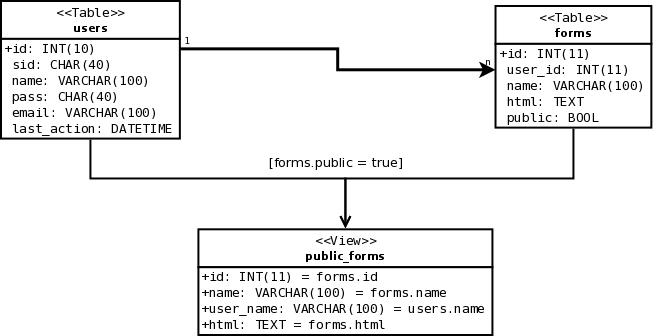
\includegraphics[width=328px]{db.png}
  \caption{Adatbázis-szerkezet}\label{fig:db}
\end{figure}

% users tábla
\subsubsection{\texttt{users} tábla}
A \texttt{sid} és \texttt{last\_action} mezőket a felhasználók bejelentkezésének
ellenőrzésekor használjuk.

\small
\vspace{.3cm}
\begin{tabular*}{\textwidth}{>{\tt}l>{\tt}l>{\tt}l>{\tt}l|l}
  \rm Név       &  \rm Típus  &  \rm Méret  & \rm Index/Kulcs & Megjegyzés           \\
  \hline
  id           &   INTEGER AUTO\_INCREMENT && PRIMARY KEY    &                      \\
  sid          &   CHAR      & 40          &                 &  PHP session cookie  \\
  name         &   VARCHAR   & 30          & INDEX           &                      \\
  pass         &   CHAR      & 30          &                 &  SHA1 hash (hex)     \\
  email        &   VARCHAR   & 100         & INDEX           &  Nem nyilvános       \\
  last\_action &   DATETIME  &             &                 &
\end{tabular*}
\normalsize

% forms tábla
\subsubsection{\texttt{forms} tábla}

A \texttt{user\_id} mezővel kapcsoljuk az űrlapot a létrehozó felhasználóhoz. A
\texttt{html} mező tárolja magát az űrlapot (a \texttt{<form>} elem nélkül), míg
a \texttt{public} mező adja meg, hogy az űrlap megjelenhet-e a nyilvános űrlapok
listáján.

\small
\vspace{.3cm}
\begin{tabular*}{\textwidth}{>{\tt}l>{\tt}l>{\tt}l>{\tt}l|l}
  \rm Név    & \rm Típus &  \rm Méret  & \rm Index/Kulcs & Megjegyzés\\
  \hline
  id        & INTEGER AUTO\_INCREMENT && PRIMARY\_KEY   &                            \\
  user\_id  & INTEGER   & 11          & INDEX           & $1..n \rightarrow{}$ users \\
  html      & TEXT      &             &                 &                            \\
  public    & BOOL      &             & INDEX           &
\end{tabular*}
\normalsize

%Tördeléskor, nem tartalmi szempont miatt
\clearpage

% public_forms nézet
\subsubsection{\texttt{public\_forms} nézet}

Megkönnyíti a nyilvános űrlapok kiválasztását, és lehetőséget ad az
adatbázismotornak az optimalizálásra. A nyilvános űrlapokat listázza
azonosítójukkal, nevükkel, a létrehozó felhasználó nevével és az űrlap
tartalmával. A MySQL adatbázis-rendszer támogatja az írható nézeteket, de számos
más rendszer nem, így ezt a nézetet csak olvasásra használjuk.

\small
\vspace{.3cm}
\begin{tabular*}{\textwidth}{>{\tt}l>{\tt}l>{\tt}l|>{\tt}l}
  \rm Név     &  \rm Típus    &  \rm Méret  & Megjegyzés \\
  \hline
  id         &  INTEGER      &  11         & forms.id   \\
  name       &  VARCHAR      &  100        & forms.name \\
  user\_name &  VARCHAR      &  100        & users.name \\
  html       &  TEXT         &             & forms.html
\end{tabular*}
\normalsize
% ----- Adatbázis-szerkezet vége -----


\phantomsection
\subsection{Modellek}
\label{sec:modellek}

A CodeIgniter a modelleket a \texttt{system/application/models} mappában
tárolja. Az alkalmazás két modellt használ: egyet a felhasználók kezelésére
(\texttt{user\_model}) és egyet az űrlapok kezelésére (\texttt{forms\_model}). A
\texttt{user\_model} csak a \texttt{users} táblát, míg a
\texttt{forms\_model} szükségszerűen mindkét táblát és a \texttt{public\_forms}
nézetet is használja.

A lekérdezések összeállításához és futtatásához a CodeIgniter ActiveRecord
szolgáltatását használjuk. Ezzel egy tipikus lekérdezés a következőképpen
valósul meg:

\begin{lstlisting}[language=PHP]
function get_form_public($id)
{
  // WHERE feltetel asszociativ tombben
  $where = array('id' => $id);

  // Lekerdezes es eredmeny
  $this->db->from('public_forms')->where($where);
  $result = $this->db->order_by('id')->get();

  // Nincs ilyen azonositoju publikus urlap
  if ($result->num_rows() == 0)
  return false;

  $row = $result->row();

  $user = $this->user->get_user(false);

  // Ha van bejelentkezett felhasznalo...
  if ($user !== false)
  // Es az ove az urlap, tudatjuk a hivoval
  $row->owner = ($user->name == $row->user_name);

  // Visszaadjuk az eredmenyt
  return $row;
  // TODO kivenni: $ (hogy LaTeX hilight boldog legyen)
}
\end{lstlisting}
\vspace{.8cm}

\phantomsection
\subsubsection{\texttt{user\_model}}

\paragraph{Regisztráció}
Itt történik a felhasználók regisztrálásához, valamint ki- és bejelentkezéséhez
szükséges adatbáziskezelés. Új felhasználó regisztrációjakor ellenőrizni
kell, hogy a megadott felhasználónév és e-mail szerepel-e a már az
adatbázisban. Az e-mail ellenőrzését a \texttt{check\_email}, a felhasználónév
ellenőrzését pedig a nem túl szerencsés nevű \texttt{not\_available} függvény
végzi. A \texttt{register} függvény csak akkor kerül meghívásra, ha már
meggyőződtünk a kapott adatok helyességéről (ld. \ref{sec:reg_check} \textit{Manager -
Regisztráció}).

Az e-mail címet jelenleg nem használjuk fel, de későbbi fejlesztéseknél szükség
lehet rá.

A \texttt{get\_user} függvény a bejelentkezett felhasználó adatait, vagy ennek
hiányában a \texttt{false} értéket adja vissza. Ha van bejelentkezettt
felhasználó, akkor itt futtatjuk az \texttt{update\_last\_action} függvényt,
ezzel biztosítva, hogy minden műveletnél frissítjük a felhasználó
bejelentkezését.

\paragraph{Bejelentkezés}
Ennél az alkalmazásnál a biztonság nem elsődleges szempont, de
így is szükség van a felhasználók bizonyos szintű védelmére. A jelszavakat és
a bejelentkezett felhasználó PHP-től kapott munkamenet-azonosítóját (session
id\cite{PHP-SID}) egyirányű titkosítás után tároljuk - előbbit a
\texttt{users.pass}, utóbbit a \texttt{users.sid} mezőben.

A felhasználónév és jelszó ellenőrzése a \texttt{login} függvényben
történik. Sikeres bejelentkezés esetén, tehát ha a megadott név/jelszó páros
szerepel az adatbázisban, az adott rekordban eltároljuk az aktuális munkamenet
azonosítóját (titkosítás után). A bejelentkezés sikerességéről a visszatérési
értékkel értesítjük a hívót.

A modellben elvárjuk az alkalmazás többi részétől, hogy minden művelet
elvégzésekor meghívja az \texttt{update\_last\_action} függvényt. Ezzel az
aktuális munkamenethez tartozó \texttt{users.last\_action} mező értékét a
jelenlegi időpontra állítjuk. Sikeres bejelentkezéskor is frissítjuk a dátumot.

\paragraph{Kijelentkeztetés}
A felhasználót csak akkor tekintjük bejelentkezettnek, ha a
munkamenet azonosítója szerepel az adatbázisban, és a hozzá tartozó utolsó
művelet nem régebbi egy napnál. A felhasználó kézi kijelentkezése esetén a
\texttt{logout} függvényben töröljük a munkamenet-azonosítót (üres sztringre
állítjuk).


\phantomsection
\subsubsection{\texttt{forms\_model}}

Ebben a modellben az űrlapok létrehozását, mentését, törlését, átnevezését és
listázását kezelő függvények szerepelnek. Az olvasás jellegű műveletek
visszatérési értéke vagy a lekérdezés eredménye, vagy (eredménytelen lekérdezés
esetén) \texttt{false}. Az írás jellegű műveletek eredménye mindig \texttt{true}
vagy \texttt{false}, a művelet sikerességétől függően.

Másik szempontból csoportosítva beszélhetünk nyilvános és privát műveletekről. A
privát műveletek csak bejelentkezett felhasználók számára elérhetőek - a
felhasználói felület szintjén is, de ha eljut egy hívás a modellig,
a futás bejelentkezett felhasználó hiányában hibával megáll. Két kivétellel az
összes függvény privát: a \texttt{get\_form\_list\_public} és a
\texttt{get\_form\_public} függvények csak publikus űrlapokkal dolgoznak. Itt
használjuk ki a \texttt{public\_forms} nézetet.


\phantomsection
\section{Manager}

A webes felület a modellek, vezérlők (controller), nézetek (view) és nyelvi fájlok
együttműködéséből áll össze. Ezért egy-egy fájl helyett több fájl bizonyos
részei alkotnak logikai egységet. Az egységek általában a felhasználó által
végezhető művelet vagy műveletek kezelését és az eredmény megjelenítését foglalják
magukban. Ezeken a művelet-központú egységeken kívül bemutatásra kerül a
felhasználóbarát URL-ek használatát lehetővé tevő rendszer, a vezérlők alaposztálya
és az új fordítások hozzáadásának módja is. Sok függvény elfogad egy opcionális
\texttt{\$lang} paramétert, aminek az alapértelmezett értéke \texttt{null}. Ez a
felhasználói felület kívánt nyelvét jelöli.

A Managerhez tartozó fájlok:

\begin{itemize}
\fitem{css/style.css, css/login.css, css/my\_forms.css} a mindenhol
  megjelenő elemekre, a bejelentkező oldalra, illetve az űrlapok listájára
  érvényes stíluslapok
\fitem{img} a \texttt{famfamfam, famfamfam\_silk} és \texttt{tango}
  mappák tartalma az adott projectből származik. A \texttt{header.jpg,
    valid.jpg} és \texttt{error.jpg} fájlokat a GIMP képszerkesztővel
  készítettem.
\fitem{scripts/login.js} a bejelentkező és regisztráló oldalhoz tartozó
  JavaScript kód (ld. \ref{sec:reg-client} \textit{Builder - Regisztráció,
    Kliensoldal})
\fitem{scripts/forms\_table.js} az űrlapok listáihoz tartozó JavaScript kód
\fitem{system/appliaction/controllers} a vezérlőket tartalmazó mappa
\fitem{system/appliaction/models} a modelleket tartalmazó mappa
(ld. \ref{sec:modellek} \textit{Builder - Modellek})
\fitem{system/application/views} a nézeteket tartalmazó mappa
\fitem{system/application/languages} a nyelvi fájlokat tartalmazó mappa
  (ld. \ref{sec:manager-i18n} \textit{Manager - Új fordítások hozzáadása} és
  \ref{sec:builder-i18n} \textit{translations.js - fordítások})
\end{itemize}

\phantomsection
\subsection{Routing - felhasználóbarát URL-ek}

A CodeIgniter framework routing\cite{CI-Routing} szolgáltatásán keresztül
könnyen használhatunk felhasználók számára is könnyen olvasható URL-eket.
A framework a futtatandó függvényt a következő módon olvassa ki az oldal
címéből: \texttt{példa.com/vezérlő/függvény/paraméter1/paraméter2}.
A \texttt{system/application/config/routes.php} fájlban megadhatunk más,
tetszőleges címeket, amiket aztán az előbbi formátumú URI-khez rendelünk. Az
URL-ek megadásánál használhatunk reguláris kifejezéseket\cite{regex}, így szinte
bármilyen helyzetnek megfelelő szabályokat fel tudunk állítani. A használt
beállítások:

\begin{lstlisting}[language=PHP, firstnumber=46]
$langs = '(en|hu)';

$route[$langs]           = 'home/index/$1';
$route['(:any)/'.$langs] = '$1/index/$2';
$route['logout']         = 'login/logout';
$route['builder/(:num)'] = 'builder/open/$1';
// TODO kivenni: $ (hogy LaTeX hilight boldog legyen)
\end{lstlisting}

A 46. sorban egy reguláris kifejezés segítségével megadjuk azokat a
nyelv-azonosítókat, amik szerepelhetnek érvényes címekben. Ezeknek az
azonosítóknak meg kell egyezniük a nyelvi fájlokban használt azonosítókkal
(ld. \ref{sec:manager-i18n} \textit{Manager - Új fordítások hozzáadása} és
\ref{sec:builder-i18n} \textit{translations.js - fordítások})

Az alábbi táblázatban az átirányítási szabályokra szerepel egy-egy példa. A
``pelda.com'' a \texttt{system/application/config/config.php} fájlban megadott
\texttt{base\_path} érték.

\vspace{.4cm}
\begin{tabular*}{\textwidth}{>{\tt}l|>{\tt}r>{$\rightarrow$}c>{\tt}l}
  \rm Sor & \rm Honnan           & & \rm Hova        \\
  \hline
  48      & pelda.com/hu         & & pelda.com/home/index/hu  \\
  49      & pelda.com/teszt/hu   & & pelda.com/teszt/index/hu \\
  50      & pelda.com/logout     & & pelda.com/login/logout   \\
  51      & pelda.com/builder/20 & & pelda.com/builder/open/20
\end{tabular*}


\phantomsection
\subsection{BaseController - a vezérlők alaposztálya}

A \texttt{system/application/controllers/BaseController.php} fájlban található
osztályban összegyűjtöttem azokat a függvényeket és beállításokat, amelyekre
bármelyik vezérlőben szükség lehet.

\paragraph{\texttt{render(\$return=false)}}
Mivel a Builderen kívül minden oldalon megtalálhatóak bizonyos
elemek - a fejléc, a menü, a lábléc - logikus lépés volt ezeknek az állandó
elemeknek egy nézetbe foglalása. A CodeIgniter lehetőséget ad rá, hogy a
nézetet betöltő függvénynek átadjunk egy tömböt, aminek a tartalma elérhető lesz
a nézetből - a kulcsok lesznek a változók nevei, az értékek pedig értelemszerűen
a tömb értékei.

Az állandó elemeket tartalmazó, \texttt{render} függvény által megjelenített
\texttt{skeleton} nézetnek a vezérlő \texttt{slots} nevű tulajdonságát adjuk
át. Így a megjelenítendő elemeket a vezérlő futása során bármikor
módosíthatjuk. Az aktuális oldal tartalmát a \texttt{slots} tulajdonság
\texttt{content} kulcsához rendeljük. Ez általában egy másik nézet futtatásának
eredménye, amit nem megjelenítettünk, hanem egy változóban tároltunk. A
\texttt{render} függvény \texttt{\$return} paramétere is ezt a célt szolgálja -
ha értéke \texttt{true}, akkor az eredményt megjelenítés helyett visszaadjuk a
hívó függvénynek.

Még a tényleges megjelenítés előtt felépítjük a menüt a \texttt{build\_menu}
függvény és a \texttt{menu} nézet segítségével, majd ha van a vezérlő nevével
megegyező nevű JavaScript, illetve CSS fájl, ezeket is átadjuk a
\texttt{skeleton} nézetnek.

\paragraph{\texttt{check\_login(\$redirect='my\_forms')}}
Ez a függvény ellenőrzi, hogy van-e bejelentkezett felhasználó, és ha nincs,
akkor átirányítja a felhasználót a bejelentkező olralra. Onnan sikeres
bejelentkezés vagy regisztráció után a \texttt{\$redirect} paraméterben tárolt
oldalra fog kerülni.

\paragraph{\texttt{remote\_check\_rights}}
\label{par:check_rights}

Ezt a függvényt AJAJ kérésekkel hívjuk a felhasználó jogainak ellenőrzése
céljából. A POST adatokból a \texttt{write} és az \texttt{id} paramétereket
olvassa be. A \texttt{write} a végzendő művelet típusára utal - ha
\texttt{true}, akkor írni, ha \texttt{false}, akkor olvasni akarunk.
Az \texttt{id} paraméter a módosítani vagy olvasni kívánt űrlap azonosítója.
A lehetséges eredmények:

\desc
  \item[OK:] A felhasználónak van joga a megadott művelethez
  \item[NOT\_LOGGED\_IN:] A kért művelethez bejelentkezett felhasználóra van szükség
  \item[FORM\_NOT\_FOUND:] A felhasználónak nincs joga kért művelethez, vagy az űrlap
    nem található.
\ed

Az eredmény kiválasztásának folyamatát a következő ábra mutatja be.

\begin{figure}[h]
  \centering
  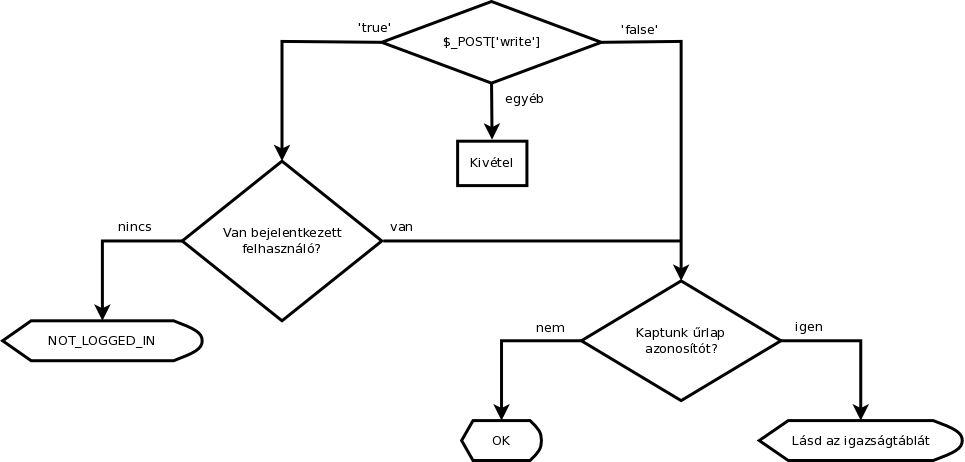
\includegraphics[width=400px]{rights.png}

  \desc\small
    \item[WRITE:] A POST-ban kapott \texttt{write} paraméter
    \item[PRIV:] Az űrlap az éppen bejelentkezett felhasználóhoz tartozik?
    \item[PUB:] Az űrlap publikus?
  \ed\normalsize

  \begin{tabular*}{\textwidth}{r|cc|cc}
    \multirow{2}{*}{WRITE} & \multicolumn{2}{c|}{PRIV = 1} & \multicolumn{2}{c}{PRIV = 0} \\
    & PUB = 1 & PUB = 0 & PUB = 1 & PUB = 0 \\
    \hline
    true  & OK & OK & NOT\_FOUND & NOT\_FOUND \\
    false & OK & OK & OK         & NOT\_FOUND \\
  \end{tabular*}

  \caption{Felhasználói jogok ellenőrzése}\label{fig:rights}
\end{figure}


\paragraph{\texttt{load\_lang(\$file, \$in=null)}}
Betölti a kért nyelvi fájlt a megfelelő nyelvi fájlból. Az \texttt{\$in}
paraméter a vezérlőkben megjelenő \texttt{\$lang} opcionális paraméter értékét
kapja. Ha tehát az URL-ben szerepel egy nyelv, akkor itt töltjük be az annak
megfelelő sztringeket. Ezen kívül elmentjük a munkamenetbe a nyelvet, amit akkor
használunk, ha az URL-ből nem kaptunk nyelvet. Ha még a munkamenetben sincs
mentett nyelv, akkor a konstruktorban megadott első nyelvet használjuk, és
mentjük is a munkamenetbe.


\phantomsection
\subsection{Új fordítások hozzáadása}
\label{sec:manager-i18n}

A felhasználói felület nyelvi fájljait a Manager és a Builder külön tárolja: a
Manager a \texttt{system/application/language} mappában, a Builder pedig a
\texttt{scripts/builder/translations.js} fájlban. Egy új nyelv hozzáadása a
Managerhez négy lépésből áll:

\begin{itemize}
  \item \textbf{A nyelv azonosítójának kiválasztása.} Általában a legegyszerűbb az
    \texttt{img/famfamfam/png} mappában található zászló nevével megegyező
    azonosítót választani. Ez a spanyol nyelv esetén például
    \texttt{es}. Ellenkező esetben a zászlóról készíteni kell egy
    másolatot, aminek a neve megegyezik az azonosítóval, hiszen a nyelvek
    kiválasztását lehetővé tevő menü ezt a képet fogja használni.
  \item \textbf{A Manager felületének lefordítása.} Egy már létező fordítás fájljait
    (például a \texttt{system/application/language/hu} mappa tartalmát)
    lemásoljuk az új nyelv azonosítójával megegyező nevű mappába, majd
    elvégezzük a fordítást.
  \item A \texttt{BaseController} osztály konstruktorában a
    \texttt{\$this->lang\_names} tömbhöz hozzáadjuk az új nyelv azonosítóját és
    nevét. Például az angol, magyar és spanyol nyelvekkel a tömb a következő
    értéket kapná:
    \begin{lstlisting}[firstnumber=35]
$this->lang_names = array('en' => 'English',
                          'hu' => 'Magyar',
                          'es' => 'Espanol'
                         );
// TODO kivenni: $ (hogy LaTeX hilight boldog legyen)
    \end{lstlisting}
    Így az új nyelv be fog kerülni a nyelv kiválasztását lehetővé tevő menübe.
  \item A \texttt{system/application/config/routes.php} fájlban a
    \texttt{\$langs} változóhoz hozzáadjuk a nyelv azonosítóját. Például az
    angol, magyar és spanyol nyelvekkel a változó a következő értéket kapná:
    \begin{lstlisting}[firstnumber=46]
$langs = '(en|hu|es)';
// TODO kivenni: $ (hogy LaTeX hilight boldog legyen)
    \end{lstlisting}
    Így a \texttt{``*/es''} alakú oldalak megnyitásakor ``Az oldal nem található''
    hiba helyett spanyol nyelven nyílik meg a kért oldal.

\end{itemize}

Ezen kívül még le kell fordítani a Builder felületének üzeneteit is (ld.
\ref{sec:builder-i18n} \textit{translations.js - fordítások}).

\phantomsection
\subsection{Regisztráció}
\label{sec:reg_check}

Az adatbázis módosítását a \texttt{users\_model} hajtja végre. A feladatunk itt
a felhasználó által megadott adatok ellenőrzése. Ellenőrizni
kell a megadott felhasználónév és e-mail cím létezését. Figyelni kell az e-mail
cím helyességére, a két jelszó-mező tartalmának megegyezésére, valamint a kapott
adatok hosszára - ennek egy megadott minimum hossz és az adatbázisban
meghatározott maximális hosszúság közé kell esnie.

Az adatok ellenőrzésére, illetve ezekről visszajelzés küldésére négy
lehetőségünk van:

\paragraph{Csak szerveroldali ellenőrzés}
Az űrlap kitöltése után közvetlenül a szervernek küldjük az adatokat, majd egy
újragenerált lapon értesítjük a felhasználót a regisztráció sikerességéről.
Hibásan küldött űrlap esetén a kapott adatokkal feltöltve írjuk ki újra az
űrlapot. Ennek a megoldásnak a megvalósítását jelentősen megkönnyíti a
CodeIgniter framework Validation osztálya\cite{CI-Val}. A felhasználónak meg
kell várnia az új lap letöltését, és kitöltés közben nem kap visszajelzést a
megadott adatok helyességéről.

\paragraph{Csak kliensoldali ellenőrzés}
A felhasználó szempontjából kényelmes, hiszen azonnali visszajelzést kap a
megadott adatokról, ráadásul a lap újratöltésére sem kell várnia hiba
esetén. Biztonsági szempontból azonban elfogadhatatlan megoldás, hiszen egy
esetleges támadónak elég egy hibás kérést küldenie az adatbázis közvetlen
eléréséhez. Ráadásul a kliensoldali ellenőrzés visszajelzéseiből megtudja, hogy
milyen adatokkal tud hibát okozni.

\paragraph{Önálló ellenőrzés a szerveren és a kliensen}
A fenti módszerek előnyeit egyesíti, hátrányaikat kiküszöböli. A kliensoldali
ellenőrzés miatt a felhasználó számára kényelmes, a szerveroldali ellenőrzés
miatt biztonságos. Könnyű kezelni azt az esetet is, ha a kliens nem tudja
futtatni az ellenőrzést (pl. a böngészőben le van tiltva a JavaScript
futtatása). Hátrány, hogy minden ellenőrzést implementálni kell mind
a szerveren, mind a kliensoldali nyelven. Így felesleges redundanciát vezettünk
be - az ellenőrzési kritériumok változásait két helyen kell módosítani, kétszer
kell tesztelni.

Ez a fajta probléma elkerülhető némi metaprogramozás bevezetésével, például a
CodeIgniter által használt kritérium-leírásokhoz hasonló nyelvvel
\cite{CI-Val}. Ha a szerveren és a kliensen futó ellenőrzés is ugyanazt a
szabályleíró fájlt használja, akkor elkerültük az ellenőrzendő esetek
ismétlését. A redundancia így átkerül a szabályleírást értelmező programrészbe,
ami valószínűleg bonyolultabb, mint maguk az ellenőrzések. Nagy számú
ellenőrzésnél ez jó megoldás lehet, de ennél az alkalmazásnál nem kifizetődő.

\paragraph{Szerveroldali ellenőrzés és AJAJ}
AJAJ-nak az AJAX (Asynchronous JavaScript and XML \cite{ajax}) technológia egy
olyan változatát nevezzük, ahol az adatok továbbítása XML helyett JSON
(JavaScript Object Notation \cite{json}) formátumban történik. Így kisebb
sávszélességet használunk, és a kliensoldalon az adatok feldolgozása egyszerűbbé
válik (bár a jQuery library képes XML-ből is JavaScript objektumokká alakítani a
kapott adatokat).

A tényleges ellenőrzést ennél a megoldásnál a szerveren végezzük, és lehetővé
tesszük, hogy a felhasználói felület szerkesztés közben a szervert megkérje
egyes adatok ellenőrzésére. Így az előző megoldás redundanciáját kiküszöböltük
néhány bájt hálózat-forgalom ellenében. A szerver terhelése így valamivel nő, de
az alkalmazás méreténél fogva valószínűsíthető, hogy nem fognak
skálázhatósági problémák fellépni.

Kérdés viszont, hogy az űrlap elküldését hogyan valósítsuk meg.
A kliensoldali ellenőrzések aszinkron volta miatt a legegyszerűbb módszer, az
űrlap \texttt{onsubmit} eseményének használata nem megoldható: visszatérési
értékre volna szükség, amit AJAJ hívásnál nem kapunk. Az eredmények
összegyűjtése utáni küldés nem megoldás, hiszen előfordulhat, hogy közben a
felhasználó még módosít az űrlapon. Lehetőség van szinkron, blokkoló módon
futtatni az ellenőrzéseket, de a mai böngészők ilyenkor a kérés teljesítéséig
nem fogadnak semmilyen felhasználói utasítást.

Ezt a problémát a csak szerveroldali ellenőrzésnél hátrányosként említett módon
oldottam meg: hiba esetén a regisztrációs oldal újra letöltődik. Mivel a
beviteli mezők szerkesztésekor az \texttt{onchange} eseményre induló ellenőrzés
jelzi a felhasználónak a megadott adatok helyességét, ez ritkán fog előfordulni.

\phantomsection
\subsubsection{Szerveroldal}

% Registration check folyamatábra
\begin{figure}[htp]
  \centering
  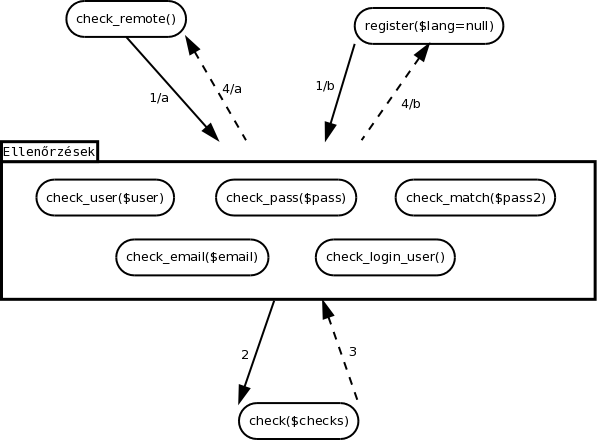
\includegraphics[width=328px]{reg_check.png}
  \caption{Regisztrációs adatok ellenőrzése}\label{fig:reg_check}
\end{figure}

%TODO: idáig van ellenőrizve

Az regisztrációnál megadott adatok ellenőrzése két helyről indulhat. Ha a kliens
kérte az ellenőrzést, akkor a \texttt{check\_remote} függvényen keresztül hívjuk
meg a kért ellenőrzést (\emph{1/a}). Ha a felhasználó már elküldte az űrlapot,
akkor a \texttt{register} függvény lefuttatja az összes ellenőrzést
(\emph{1/b}). Az \texttt{Ellenőrzések} a kapott adatok biztonságossá tétele után a
\texttt{check} függvényen keresztül végzik el az adatok tényleges ellenőrzését
(\emph{2, 3}), majd visszaadják az eredményt a hívó függvénynek (\emph{4/a, 4/b}).


\paragraph{\texttt{check(\$checks)}}
Ez a függvény megkönnyíti az ellenőrzések elvégzését, a hozzájuk szükséges kódot
lerövidíti. A \texttt{check\_*} függvények előkészítik számára az ellenőrzéseket
egy-egy sztring formájában, ami a futtatandó ellenőrzést tartalmazza PHP kód
formájában. Ezekben az ellenőrző kódokban a vezérlőt (controller) a
\texttt{\$controller} változón keresztül lehet elérni. Erre például a
felhasználónév létezésének ellenőrzésénél van szükség.

A kapott paraméter egy asszociatív tömb, ahol a kulcs a futtatandó ellenőrzés,
az érték pedig egy vektor: a hiba esetén megjelenítendó üzenet azonosítója és
az abba behelyettesítendő értékek. Az üzenet tényleges szövegét az aktuális
nyelvnek megfelelő nyelvi fájlból fogjuk kiolvasni. A behelyettesítendő érték
lehet például nem megfelelő hosszúságú adatnál a minimális vagy maximális
megengedett hosszúság.

A ténylegesen futtatott
ellenőrző-függvényt a \texttt{create\_function} függvénnyel hozzuk létre. Ha
például a kapott ellenőrző kód:
\texttt{"\$controller->user->not\_available('foo')"}, akkor a létrehozott
függvény a következő:

\begin{lstlisting}[language=PHP, numbers=none]
function lambda($controller)
{
  return ($controller->user->not_available('foo'));
}
\end{lstlisting}

A függvénynek a \texttt{\$controller} paraméterbe a \texttt{\$this} értékét
adjuk át, ezzel biztosítva a hívó vezérlő elérhetőségét az ellenőrzésen
belül. Ha az így létrehozott és futtatott függvény visszatérési értéke
\texttt{false}, akkor az ellenőrzéshez tartozó üzenetleíró vektort hozzáadjuk a
hibák listájához, amit aztán az összes ellenőrzés lefuttatása után visszaadunk a
hívó függvénynek.


\paragraph{\texttt{Ellenőrzések}}
Az \texttt{check\_} prefixumú függvények egyetlen paraméterükként az
ellenőrzendő értéket várják. Még a \texttt{check\_pass\_match} függvény is, ami
a megadott jelszavak ellenőrzését végzi - itt az egyik jelszót a POST adatokból
olvassuk ki. Mivel az ellenőrzendő és a hiba esetén újra kitöltendő mezők neve
ugyanazon tömbben szerepel, és a bejelentkezési űrlap nevét nem ellenőrizzük
változtatásakor, a \texttt{check\_login\_user} függvény mindig egy üres tömböt
ad vissza - ezzel jelezve, hogy nincsenek hibák.

Az adott ellenőrzésekre jellemző adatok (például minimum és maximum hosszúság)
beállítása után a vizsgálni kívánt adatokban a \texttt{'} karaktereket
\texttt{\textbackslash'}-re cseréljük, mivel az ellenőrzéseket először sztringekként állítjuk
össze. A cserével kivédjük a SQL injectionhöz hasonló támadásokat.

Végül a szükséges ellenőrzéseket és hozzájuk tartozó hibaüzeneteket átadjuk a
\texttt{check} függvénynek, aminek az eredményét feldolgozás nélkül visszaadjuk
a hívónak. Itt nem dolgozzuk fel a hibaüzeneteket, hiszen nem tudhatjuk, hogy a
hívó függvény hogyan kívánja értesíteni a felhasználót, vagy az őt hívó
függvényt.


\paragraph{\texttt{check\_remote}}
Ezt a függvényt érik el a kliens ellenőrzési kérései egy POST hívás
segítségével. Egy hívás pontosan egy mező ellenőrzését kéri, tehát pontosan egy
\texttt{check\_*} függvény futását fogja eredményezni. Ha visszakapott, hibákat
tartalmazó tömb üres, akkor a \texttt{true} sztringet írjuk ki, ami JSON-ként
való értelmezés után a \texttt{true} bináris értéket fogja képviselni a
kliensoldalon.

Ha vannak hibák, akkor a hozzájuk tartozó üzenetet adjuk vissza idézőjelek
között - így a JSON értelmezése után a kliensoldalon is sztringet kapunk. Ha
több hiba van, akkor is csak az elsőt adjuk vissza. Ha például egy kötelezően
kitöltendő mező üres, akkor elég csak a ``Kitöltés kötelező'' üzenetet kiírni, a
``Legalább 5 karakter hosszú legyen'' figyelmeztetés felesleges.


\paragraph{\texttt{register(\$lang=null)}}
Ez a függvény kezeli az elküldött regisztrációs űrlapot. Lefuttatja az összes
ellenőrzést, és ha bármelyik hibával tér vissza, visszaküldi a felhasználót a
regisztrációs oldalra a felhasználónév és e-mail mezők értékét feltöltve a
felhasználó által megadottakkal.

Ha nincs hiba, \texttt{user\_model} \texttt{register} függvényén keresztül
elvégzi az ellenőrzést, és a POST adatok között kapott \texttt{redirect} oldalra
irányítja a felhasználót.


\subsubsection{Kliensoldal}
\label{sec:reg-client}

A kliens feladata csupán annyi, hogy szerkesztéskor, illetve hibás űrlap küldése
után elvégeztesse a szerverrel a megfelelő ellenőrzéseket, és megjelenítse az
eredményt a felhasználó számára.

Az ellenőrzés meghívását és az eredmény kezelését a \texttt{check\_ajaj}
függvény végzi. A jQuery framework segítségével elküldi a \texttt{data}
paramétert a fenti \texttt{check\_remote} függvénynek, majd az eredménynek
megfelelő képet és üzenetet helyez el az \texttt{\$input} paraméterben kapott
beviteli mező után. A Builderben is megjelenő \$ prefixumú változónevek arra
utalnak, hogy a tárolt érték egy jQuery objektum. Ha a \texttt{check\_ajaj}
függvény \texttt{initial} paramétere \texttt{true}, akkor az üres mezőknél is
megjelenítjük a hibaüzeneteket. Ez csak közvetlenül az oldal betöltődése után
fordul elő, és az üresen elküldött mezők jelölésére szolgál.

A \texttt{check} függvény a \texttt{name} paraméterben átadott mező értékének
ellenőrzésére szolgál. Eltávolítja az előző ellenőrzések eredményeit az
űrlapról, majd a mező értékéből és a \texttt{name} paraméterből összeállított
\texttt{data} paraméterrel meghívja a \texttt{check\_ajaj} függvényt. Az
\texttt{\$input} paraméterbe értelemszerűen az ellenőrzött beviteli mező kerül,
az \texttt{initial} értéket pedig egyszerűen továbbadja. A
\texttt{check\_pass\_match} függvény hasonló módon működik, de \texttt{data}
értékeit a szerveroldali \texttt{check\_pass\_match} függvénynek megfelelő
formában állítja össze.

Mindkét függvényt a beviteli mezők \texttt{onchange} eseményének futásakor és az
oldal betöltődésekor hívjuk meg.


\clearpage
\phantomsection
\subsection{Űrlapok listázása}

\begin{figure}[H]
\centering
  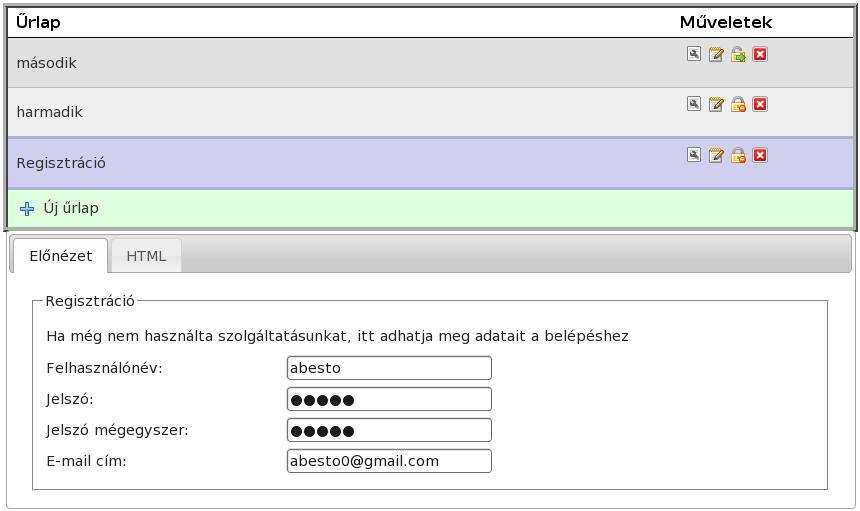
\includegraphics[width=420px]{form_list.png}
  \caption{Űrlapok listája, előnézet}
\end{figure}
\begin{figure}[H]
  
\includegraphics[width=420px]{form_list_html.png}
  \caption{Űrlap HTML nézete}
\end{figure}
\clearpage

Az ``Űrlapjaim'' és ``Nyilvános űrlapok'' menüpontból elérhető lista két részből
áll: az űrlapokat  és rajtuk végezhető műveleteket tartalmazó táblázatból,
illetve a kiválasztott űrlap előnézetéből. Az előnézet két fület tartalmaz: az
``Előnézet'' az űrlapot úgy mutatja meg, ahogyan a felhasználó böngészőjében
megjelenik; a ``HTML'' nézet pedig az űrlap forrását teszi elérhetővé.

A lista felépítése két lépésből áll. Először a \texttt{My\_forms} vagy
\texttt{Public\_forms} vezérlő
segítségével betöltjük a \texttt{form\_table} nézetet, és átadjuk neki
\begin{itemize}
\item A \texttt{public = false} értéket. Ez a nézet kezeli a nyilvános és a
  saját űrlapok megjelenítését is - így tudatjuk vele, hogy most saját
  űrlapokról van szó. Ha a változó értékét futásidőben megváltoztatják, az
  állandó jog-ellenőrzés miatt akkor sem lehet kihasználni ezt a tényt.
\item A \texttt{forms\_lang.php} nyelvi fájl \texttt{js} és \texttt{php} nevű
  tömbjeit. A tömbök neve azt jelzi, hogy melyik programnyelv fogja felhasználni
  az adott szövegrészleteket.
\item A \texttt{base\_url} CodeIgniter függvény visszatérési értékét. Ez a
  \texttt{config.php}-ben megadott \texttt{base\_url} változó értéke.
\end{itemize}

Ezután a \texttt{form\_table.php} nézetben a \texttt{js} tömb, a
\texttt{base\_url} és \texttt{public} változók értékét átadjuk a
JavaScriptnek. Végül a \texttt{php} tömb lefordított sztringjeit felhasználva
létrehozzuk a felhasználói felület részeit.

\vspace{1cm}

A második lépésben AJAJ-al lekérdezzük a felhasználó űrlapjainak
a listáját, amiket JavaScripttel megjelenítünk. Az űrlap táblázathoz adására
itt is ugyanazt a függvényt használjuk, mint új űrlap létrehozásakor. Ezt,
illetve az űrlapokon végezhető műveletek kezelését a
\texttt{scripts/forms\_table.js} végzi.

Az új sor hozzáadását két függvény végezheti: az \texttt{add\_row} saját űrlap
hozzáadását, az \texttt{add\_row\_public} pedig más felhasználók nyilvános
űrlapjainak hozzáadását teszi lehetővé. A vezérlőtől kapott, JavaScriptnek
átadott \texttt{public} változó értékétől függ, hogy melyiket használjuk.i

Az űrlapok táblázata a fejlécből, a létező űrlapok listájából, és a saját
űrlapok listájának esetén egy ``Új űrlap'' sorból áll. Minden űrlapnál szerepel
az űrlap neve, nyilvános űrlaplista esetén az űrlap tulajdonosának neve, és az
adott űrlapon végezhető műveletek. Ha a felhasználó nincs bejelentkezve, akkor
nincsenek műveletek. Bejelentkezett felhasználó más felhasználó nyilvános űrlapjait
szerkesztésre nyithatja meg, amit később mentés esetén sajátjaként mentünk, új
űrlapként. Saját űrlapoknál a nyilvános űrlapok listázásakor a szerkesztés,
átnevezés és törlés műveletek elérhetőek. Ezeken kívül a saját űrlapok listáján
az űrlap nyilvánosságának megváltoztatására is van lehetőség.

\begin{figure}[H]
\centering
\small
  
\includegraphics[width=420px]{private.png}
  Saját űrlap az ``Űrlapjaim'' menüpont alatt: minden művelet elérhető\\

  \vspace{.5cm}
  
\includegraphics[width=420px]{public_sajat.png}
  Saját űrlap a ``Nyilvános űrlapok'' menüpont alatt: látjuk az űrlap
  létrehozójának nevét. A nyilvánosság átállításán kívül minden művelet
  elérhető\\

  \vspace{.5cm}
  
\includegraphics[width=420px]{public_mas.png}
  Más felhasználó nyilvános űrlapja a ``Nyilvános űrlapok'' menüpont alatt: csak
  a szerkesztés menüpont érhető el. Mentéskor másolat készül a felhasználó
  sajátjaként.\\

  \vspace{.5cm}
  
\includegraphics[width=420px]{public_none.png}
  Nyilvános űrlap a ``Nyilvános űrlapok'' menüpont alatt, bejelentkezés nélkül:
  az űrlapok listája és az előnézet megtekinthető, de nincs végezhető művelet.
\normalsize
  \caption{Egy űrlap lehetséges megjelenési formái}
\end{figure}
\vspace{.7cm}


\paragraph{Előnézet, gyorsítótár}
Egy űrlap sorára - nem egy műveletre - kattintva az űrlap kijelölésre kerül. Ezt
jelezzük a sor kiemelésével, és az előnézetben a kijelölt űrlapot mutatjuk. Némi
sávszélesség megspórolása érdekében az űrlapok tartalmát nem töltjük le, amíg
nincs rájuk szükség. A kijelölt űrlap letöltése közben a felhasználó egy ``Űrlap
letöltése'' feliratú üzenetet kap. Ezután az űrlap illetve a HTML forráskód
megjelennek a megfelelő lapokon. Az adatbázisban az űrlapokat whitespace nélkül
tároljuk, ezért szükség van a kód olvashatóvá tételére. Ezt az átalakítást az
eredetileg csak a Builderben használt \texttt{scripts/builder/htmlize.js}
fájlban definiált \texttt{htmlize} rekurzív függvény végzi.

Az űrlap letöltődése utána az bekerül a \texttt{cache} nevű
gyorsítótár-objektumba. Ha az űrlapot a felhasználó később újra kijelöli, akkor
az a szerver helyett innen, a kliensgép memóriájából fog betöltődni. A
\texttt{cache} objektumnak van egy \texttt{update} tagfüggvénye is, ami az
űrlapok nevének és tartalmának módosítására szolgál. Ezt a Builder mentéskor a
\texttt{window.opener} tulajdonságon keresztül próbálja meghívni. Természetesen
ha a szerkesztőt nem az aktuális ablakból nyitotta meg a felhasználó, akkor a
gyorsítótár - és így az előnézet - nem frissül.

Ezt a gyorsítótár adott időközönként történő újratöltésével, vagy egy Comet (más
néven AJAX Push, Fordított AJAX \cite{comet}) megoldással ki lehetnek kerülni,
de jelen alkalmazásnál a befektetett munka nem lenne arányos a megoldott
probléma nagyságával.


\paragraph{Műveletek}
Az űrlapokon végezhető műveleteket tartalmozó cellában az ikonok alatt helyet
kapott egy alaphelyzetben üres \texttt{div}, ami az egérkurzor alatti ikonhoz
tartozó művelet nevét mutatja. Az ikonok létrehozására (a nyilvánosság
beállítása kivételével, ami a két állapot miatt különleges) az
\texttt{action\_icon} függvényt használjuk. A megadott képfájllal, felirattal és
űrlap-azonosítóval létrehozott kép elemet ad vissza.

Kattintásra a \texttt{check\_rights} függvénynek átadja a kapott \texttt{fun,
  write} és \texttt{id} paramétereket. Ez a vezérlő
\texttt{remote\_check\_rights} függvényét a \texttt{write} és \texttt{id}
paraméterekkel hívja (ld. \ref{par:check_rights} \textit{BaseController -
\texttt{remote\_check\_rights}}). Ha a kapott eredmény NOT\_LOGGED\_IN, akkor a
felhasználót átirányítja a bejelentkező oldalra; ha FORM\_NOT\_FOUND, akkor a
felhasználó értesítése után törli a listáról az űrlapot; ha OK, akkor lefuttatja
a \texttt{callback} paraméterben kapott programkódot (ez az
\texttt{action\_icon} függvényben a \texttt{fun} nevet viselte). Egyéb esetben
kivételt dob és a futás megáll.

A műveleteket a szerverloldalon elvégző függvények az adatbázis módosítása előtt
ellenőrzik a bejelentkezett felhasználót. A modellben is csak akkor hajtódik
végre a művelet, ha a bejelentkezett felhasználó megfelelő jogosultsággal
rendelkezik. Az űrlapokon végezhető műveletek:

\begin{itemize}
\item \textbf{Szerkesztés}: az \texttt{open\_editor} megnyitja a ``builder\_app'' nevű ablakban az űrlapot
  szerkesztésre. A Builder a lap bezárása előtt ha van mentetlen változtatás,
  rákérdez a mentésre, így nincs adatvesztés akkor sem, ha új űrlapot nyitunk meg.
\item \textbf{Átnevezé}s: az ikonra kattintva a \texttt{rename\_dialog} függvény megnyitja
  az új nevet bekérő jQuery UI párbeszédablakot. Az ott található űrlap
  elküldése után a \texttt{rename\_form} függvény elküldi a szervernek az
  átnevezést, és az űrlapok listáját is frissíti az új névvel.
\item \textbf{Új űrlap}: a \texttt{new\_dialog} függvénnyel megnyitjuk az új űrlap nevét
  bekérő párbeszédablakot, majd a \texttt{new\_form} függvénnyel azt létre is
  hozzuk. A szervernek küldött kérésre érkező válasz az új űrlap
  azonosítója. Ezt felhasználva adjuk hozzá a gyorsítótárhoz és az űrlapok
  listájához az űrlapot, majd megnyitjuk szerkesztésre a fent említett
  \texttt{open\_editor} függvény segítségével.
\item \textbf{Űrlap eltávolítása}: a \texttt{remove\_dialog} függvénnyel megnyitjuk a
  megerősítést kérő párbeszédablakot, majd a \texttt{remove\_form} függvénnyel
  azt el is távolítjuk a szerverről és az űrlapok listájáról.
\item \textbf{Nyilvánosság módosítása}: itt nem használunk párbeszédablakot. Az ikon,
  illetve ha felette van a kurzor, akkor a felirat, mutatják az aktuális
  állapotot, ami kattintásra megváltozik. Az ikont a
  \texttt{toggle\_public\_icon} függvényben hozzuk létre, amit először az \texttt{add\_row}
  függvényben hív az adatbázisban szereplő értékkel - tudnia kell a függvénynek,
  hogy mi az aktuális állapot. Kattintásra az ikon a \texttt{set\_public}
  függvényt hívja az aktuális állapot negáltjával - erre akarjuk állítani a
  nyilvánosságot. Ez a függvény elvégzi az állapot megváltoztatását a szerveren,
  majd a \texttt{toggle\_public\_icon} függvény segítségével létrehozza az új
  ikont, ami már az új állapotot mutatja, és lecseréli a régi ikont.
\end{itemize}


\phantomsection
\section{Builder}

Az alkalmazásnak ez a része teszi lehetővé az űrlapok szerkesztését.
Az űrlap az XHTML1.1 szabványnak megfelelően közvetlenül csak \texttt{fieldset}
elemeket tartalmazhat, tetszőleges számban. Ezekhez az elemekhez a felhasználó
tetszőleges számú táblázatot adhat. A táblázat egyetlen cellával jön létre,
amihez képest új cella hozható létre jobbra és balra, illetve új sor (megint
egyetlen cellával) fel- vagy lefelé. A cellák vízszintes irányban tetszőleges
módon egyesíthetőek és újra feloszthatóak.

A Builderhez tartozó JavaScript fájlokat a kisebb méret elérése érdekében
összekapcsoltam egy fájlba, majd ezt tömörítettem a YUI Compressor\cite{YUI}
segítségével. Ez azért hasznos, mert a Compressornak így rendelkezésére állnak a
függvények definíciói és hívásai is, tehát biztonságosan átnevezheti őket
(általában egy karakter hosszúságú azonosítokra). A tömörítés során ezen kívül
eltávolításra kerülnek a megjegyzések, illetve a szóköz, tabulátor és újsor
karakterek. Ezzel az összefűzött fájl mérete 51 kilobyte-ról 21 kilobyte-ra
csökkent, ezzel a letöltési időt 41 százalékkal megrövidítve.

A tömörített \texttt{scripts/builder.min.js} fájl az alábbi listán
szereplő JavaScript fájlokból jött létre, amik a \texttt{scripts\_dev/builder}
mappában találhatóak. A \texttt{htmlize.js} fájlt nem csatoltam a nagy fájlhoz,
mivel ezt a Manager is használja a HTML forrás megjelenítésekor. Ezt a
folyamatot a \texttt{scripts\_dev} és \texttt{scripts\_dev/builder} mappákban
találhato \texttt{Makefile}-ok automatizálják\cite{make}.

\begin{itemize}
\fitem{system/application/controllers/builder.php} a Builder megnyitása a kért
azonosítóval, átadva a nézetnek a szükséges adatokat
\fitem{system/application/views/builder.php} a Builder felhasználói felületének
felépítése, az űrlap megjelenítése és a JavaScriptben használt adatok
átadása
\fitem{utils.js} segédfüggvények az űrlappal történő munkához
\fitem{actions.js} az elemeken végezhető műveleteket leíró fájl
\fitem{props.js} az elemekhez tartozó tulajdonságokat leíró fájl
\fitem{builder.js} a Builder inicializálása, valamint a felhasználói felület
kezeléséért felelős függvények
\end{itemize}

\clearpage
\begin{figure}[H]
  \centering
  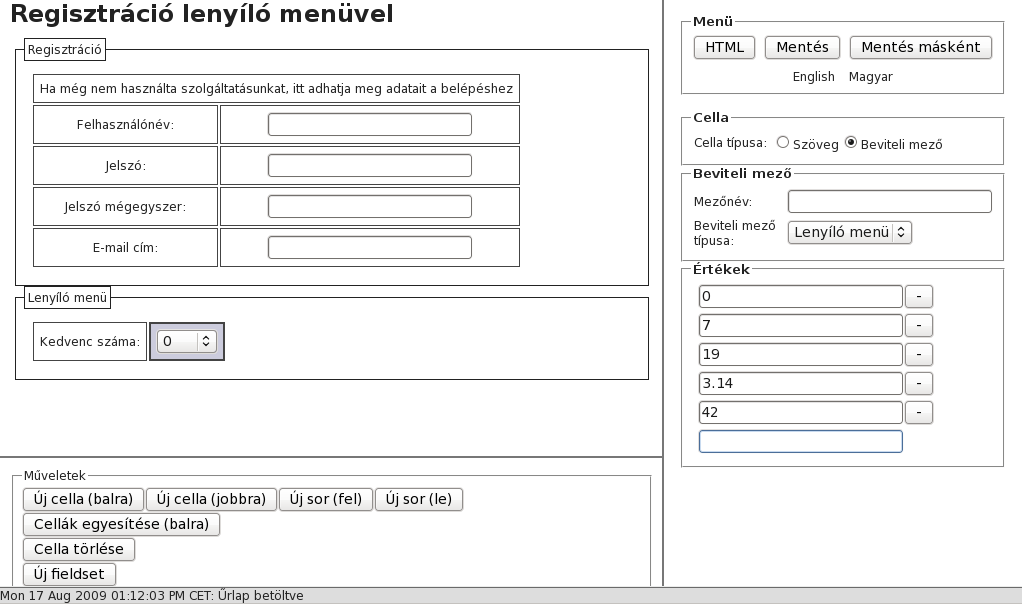
\includegraphics[width=420px]{builder.png}
  \caption{Builder felhasználói felület}\label{fig:builder}
\end{figure}

\paragraph{A felhasználói felület}
A szerkesztés az űrlap elemein értelmezett \textit{műveletek} végrehajtásán és
\textit{tulajdonságok} módosításán keresztük történik. Ha a kurzor alatti elemet
ki lehet jelölni, akkor ezt a felhasználóval az elem színének megváltoztatásával
tudatjuk. A kattintással kijelölt elemet egy másik háttérszínnel és a körvonal
megvastagításával emeljük ki. Az űrlap beviteli mezőit önmagukban nem lehet
kijelölni, csak az őket tartalmazó tábálzat-cellát. A mezőhöz tartozó
tulajdonságok az őt tartalmazó táblázat-cella tulajdonságai alatt jelennek meg.

A kijelölt elemen végezhető műveleteket az oldal alsó részén jelenítjük meg. Az
egymással kapcsolatban álló műveletek egy sorba kerülnek, ezzel átláthatóbbá
téve a felületet.

A lap jobb oldalán található legfelül a menü. A felhasználónak ezen keresztül
van lehetősége az űrlap HTML forrásának megtekintésére, az űrlap mentésére
valamint a felület nyelvének megváltoztatására. Nyelv váltásakor a felület
minden elemének felirata azonnal az új nyelvnek megfelelő szövegre változik.
A menü alatt kaptak helyet az éppen kijelölt elem tulajdonságainak módosítására
szolgáló gombok, szövegmezők. Ezeknek a hatása azonnal látszik az űrlapon,
hasonlóan sok IDE grafikus felület szerkesztésére szolgáló felületéhez.

A jQuery UI Resizable moduljának köszönhetően a menüt és a tulajdonságokat
tartalmazó sáv - az operációs rendszerek grafikus felületéhez hasonlóan - az
elválasztó mozgatásával átméretezhető. Ilyenkor az oldal többi része
alkalmazkodik az átméretezéshez, a szabadon maradt helyet használják ki.

Az oldal alján látható egy állapotsáv, ami az utolsó mentés időpnontját
mutatja. Technikailag a szerkesztés során bármikor módosíthatjuk a
feliratát. Hibák keresésekor is hasznos lehet, ha az éppen használt böngészőnek
nincsen erre használható szolgáltatása.

\clearpage
\paragraph{Műveletek és tulajdonságok}
Mivel a magához az űrlaphoz tartozó műveletek - a forrás megtekintése,
mentés, mentés másként - a menün keresztül mindig elérhetőek, az egyetlen
kivétel, az új fieldset hozzáadása mindig látható az oldal alján elhelyezkedő
Műveletek fieldsetben. A másik lehetőség az lenne, hogy az űrlapot kijelölhetővé
tesszük, és az egyetlen műveletként az új fieldset hozzáadását határozzuk meg.

A kijelölhető elemekhez tartozó műveletek és tulajdonságok:

\elem{fieldset}{Új táblázat, Fieldset eltávolítása}{Felirat}
\elem{table}{Táblázat eltávolítása}{-}
\elem{td}{
  Új cella (balra és jobbra),
  Új sor (fel és le),
  Cellák egyesítése (balra és/vagy jobbra, ha van szomszédos cella),
  Cella felosztása (balról és jobbról, ha a cella többoszlopost),
  Cella törlése
}{
  Cella típusa (szöveges vagy beviteli mező,
  Szöveg,
  Beviteli mező típusa (ha a cella típusa ``beviteli mező''
}
\elem{select}{-}{Kiválasztható értékek}
\vspace{1cm}

Minden művelet végrehajtásakor és tulajdonság módosításakor \texttt{true}ra
állítjuk a \texttt{dirty} változó értékét, amit az oldal \texttt{onBeforeUnload}
eseményére ellenőrzünk. Ha \texttt{true}, akkor a mentetlen módosításokról szóló
figyelmeztető szöveget adjuk vissza, amit a böngésző beilleszt a saját
figyelmeztető párbeszédablakába, ami az oldal elhagyásáról szól. Ha a
\texttt{dirty} változó értéke \texttt{false}, akkor az eseményre induló függvény
\texttt{null}t ad vissza, így a párbeszédablak nem jelenik meg, az oldalat a
felhasználó elhagyhatja. A \texttt{dirty} változó értékét a \texttt{remote.js}
fájl \texttt{save} és \texttt{save\_as} függvényeiben állítjuk \texttt{false}-ra,
értelemszerűen az űrlap mentésekor és új néven történő mentéskor.


\phantomsection
\subsubsection{\texttt{utils.js} - segédfüggvények}
Ez a fájl olyan függvényeket tartalmaz, amiket az alkalmazás több részében
használunk. A kényelmi funkciók mellett a következő függvények az alkalmazás
működéséhez szükséges algoritmusokat is tartalmaznak:

\begin{itemize}
\fitem{check\_selected\_type}
Szinte minden művelet és tulajdonságot kezelő
függvény használja. Ellenőrzi, hogy az éppen kijelölt elem a paraméterben
megadott típusú-e (pl. TD), és ha igen, visszaadja az elemet tartalmazó jQuery
objektumot. Ellenkező esetben hibával megállítja a futást. Az alkalmazás
helyes működése esetén ez nem fordulhat elő, hiszen a megjelenítendő
tulajdonságok és műveletek a kiválasztott elem figyelembevételével kerülnek
kiválasztásra.

\fitem{get\_td\_type}
A táblázat-cella tartalmának típusát adja vissza. Minden cellát három típusba
sorolunk: máshogyan kell kezelni a csak szöveget, a lenyíló menüt
(select) és az egyéb beviteli mezőket tartalmazó mezőket. A felhasználó nem
tud arról, hogy a lenyíló menüt ilyen szinten is megkülönböztetjük - az ő
szempontjából az is egy beviteli mező.

\fitem{set\_td\_type}
A kért típusra állítja a kijelölt mezőt. A cella szöveges tartalma a
\texttt{get\_td\_text} és \texttt{set\_td\_text} függvényeknek köszönhetően a cella
típusváltásai között megmaradhat (kivéve a \texttt{file} inputot, ahol a
szöveges tartalom nem értelmezhető).

\fitem{get\_input\_type, set\_input\_type}
Az adott cella beviteli mezőjének típusát visszaadó, illetve a kiválasztott
cella beviteli mezőjének típusát beállító függvények. Itt kezeljük a select és a
többi beviteli mező közti különbséget: ezen függvények hívójának nem kell
törődnie ezekkel a különbségekkel.

\fitem{get\_td\_text, set\_td\_text}
Az adott cella szöveges tartalmát visszaadó, illetve új szövegre állító
függvények. Itt implementáljuk a szöveges tartalmak \ref{sec:spec}
\textit{Feladatmeghatározás - Builder} részben meghatározott értelmezését. A hívó
függvénynek nem kell foglalkoznia a cella tényleges tartalmával.

\fitem{set\_name}
A paraméterként átadott cellában levő beviteli mező \texttt{name} és \texttt{id}
tulajdonságait állítja be. A \texttt{name} értéke pontosan az lesz, amit a
felhasználó megadott. Az \texttt{id} a mező egyedi azonosítására szolgál az
alkalmazás számára. A törlés következtében felszabaduló azonosítókat kiosztjuk
a később létrehozott elemeknek. Az azonosítót jelenleg nem használjuk, de a
műveletek visszavonásánál szükség lesz rá. Akadályt jelenthet az azonosítók
újrakiosztása, de ez könnyen kikapcsolható.

\fitem{status}
Az állapotsor kezeléséért felelős objektum. A \texttt{set} függvény a hívás
időpontjával és a kapott \texttt{val} paraméterhez tartozó, aktuális nyelvre
lefordított szöveget írja az állapotsorba. Az \texttt{update\_lang} függvény az
időpont frissítése nélkül frissíti a szöveget, újra beolvasva azt a fordításokat
tartalmazó objektumból. A felhasználói felület nyelvének megváltoztatásakor
hívjuk.
\end{itemize}

\phantomsection
\subsection{\texttt{actions.js} - műveletek}
Ez a fájl írja le az egyes műveletek végrehajtásának módját, illetve módot ad
rá, hogy adott elemen végezhető műveletek listáját egyszerűen lekérdezzük. A
\texttt{call\_action} függvény kizárólagos használata a műveleteket végző
függvények hívására biztosítja, hogy a mentetlen műveletek ellenőrzésére
használt \texttt{dirty} változó értéke \texttt{true} lesz egy-egy művelet
után. Ezen kívül a műveletek tervezett visszavonásánál is itt fogjuk hozzáadni a
műveletet a veremhez.

Az \texttt{ACTIONS} objektum (csupa nagybetűvel) gyakorlatilag a JavaScriptben
nem létező névtér helyettesítésére szolgál. Minden függvénye egy-egy műveletet
végez el a kiválasztott elemen. Ha a kiválasztott elem nem olyan típusú, amire a
függvénynek szüksége van, akkor a \texttt{check\_selected\_type} függvény
jóvoltából a futás hibával megáll.

Az \texttt{actions} objektum (csupa kisbetűvel) szintén egy névtérként
értelmezhető. Itt az egyes függvények a függvény nevének megfelelő elemen
végezhező műveletek listáját adják vissza. A lista minden eleme egy függvényhívást
tartalmaz szöveges formában, vagy a ``\texttt{br}'' sztringet. A felhasználói
felületen az előbbi helyére a megfelelő műveletet végző gomb fog kerülni, az
utóbbi helyére pedig egy sortörés. A sortörésekkel logikai csoportokba tudjuk
szedni a műveletek gombjait. A végezhető műveletek kiválasztásánál figyelembe
vesszük nem csak az elem típusát, de állapotát és helyzetét is - például ha egy
cella a sor bal szélső cellája, akkor a ``Cellák egyesítése balra'' művelet nem
fog szerepelni a listában.


\phantomsection
\subsection{\texttt{props.js} - tulajdonságok}
Az alapelv megegyezik a fenti \texttt{actions.js} megvalósításával, de a
műveletek és a tulajdonságok természete közti különbségek megjelennek az
alkalmazásban is. Egy művelet egyértelműen megjeleníthető egy nyomógombbal, de
egy tulajdonság megjelenítése nem automatizálható ilyen módon.

Ezért a \texttt{PROPS} névtér függvényei nem a tulajdonság módosítását végzik,
hanem egy DOM elemet adnak vissza (pontosabban egy jQuery objektumot, ami a DOM
elemet tartalmazza), ami a megfelelő események kezelőiben módosítja az éppen
kiválasztott elem megfelelő tulajdonságát.

A \texttt{props} névtér függvényeinek feladata itt is a kiválasztott elemen
értelmezhető tulajdonságok meghatározása, de itt nem elég egy egyszerű listát
létrehozni. Egy fa-szerű szerkezetre van szükség, ugyanis a különböző
csoportokhoz tartozó tulajdonságokat logikai egységekben kell
megjelenítenünk. Tekintsük a következő példát: a felhasználó kijelölt egy
cellát, amiben szerepel egy lenyíló menü. Így meg kell jelenítenünk
\desc
\item[a cella tulajdonságait:] a cella típusát (szöveges vagy beviteli mező),
  iletve a cella szövegét
\item[a beviteli mező tulajdonságait:] a mező nevét és típusát
\item mivel a lenyíló menüről van szó, a mező értékeit (illetve az új érték
  hozzáadásához és létező értékek törléséhez szükséges vezérlőket).
\ed

Ezt valósítják meg a \texttt{PropsCollection} és a \texttt{Prop} osztályok. A
\texttt{Prop} objektum csak egy gyűjtemény a művelet tulajdonságairól - a nyelvi
fájlban szereplő leírás azonosítóját és a megjelenítendő DOM elemeket
tartalmazza. A \texttt{PropsCollection} osztály két tömbből és az ezeket
manipuláló függvényekből áll. A \texttt{groups} vektor az objektumhoz hozzáadott
csoportok listáját tartalmazza. A lista elemei a nyelvi fájlban lefordított,
adott csoportot leíró szövegek azonosítói. Ezen kívül ugyanezek az értékek a
kulcsai a \texttt{PropsCollection} objektum \texttt{props} tömbjének is. Minden
helyen egy vektor szerepel, aminek elemei a tulajdonságokat leíró \texttt{Prop}
objektumok.

\begin{figure}[H]
  \centering
  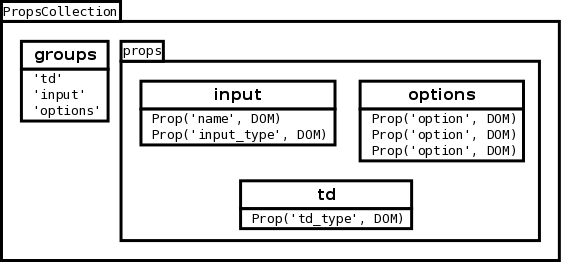
\includegraphics[width=420px]{PropsCollection.png}
  \caption{Tulajdonságok gyűjteménye, ha a kijelölt cella egy lenyíló cellát
    tartalmaz, ami két elemmel van feltöltve. A harmadik elem az üres mező,
    amivel új elemet vehet fel a felhasználó.}\label{fig:props_collection}
\end{figure}


\phantomsection
\subsection{\texttt{translations.js} - fordítások}
\label{sec:builder-i18n}

A fájlban egyetlen objektum, a \texttt{TRANS} definíciója található. Az objektum
tartalmazza a Builder által használt összes szöveg fordítását minden nyelven. A
nyelvek azonosítója az objektum tulajdonságainak neve. A kulcshoz tartozó érték
egy újabb objektum, ami tartalmazza a nyelv nevét, azonosítóját és a lefordított
szövegeket. A nyelvek azonosítóin kívül a \texttt{TRANS} objektum \texttt{list}
tömbjében tároljuk az elérhető nyelvek listáját. Új fordítás hozzáadása ezek
alapján három lépésből áll:

\begin{itemize}
\item A nyelv azonosítójának hozzáadása a \texttt{TRANS.list} tömbhöz
\item Másolat készítése egy már létező nyelvről a nyelv nevének és
  azonosítójának beállításával. Az azonosítónak muszáj egyeznie a
  \ref{sec:manager-i18n} \textit{Manager - Új fordítások hozzáadása} részben leírt
  azonosítóval, és javasolt, hogy a nyelv megnevezése is ugyanaz legyen.
\item A sztringek lefordítása. Az egyes szövegek környezetének egyértelműsítése
  érdekében a sztringeket további objektumokba csoportosítottam - ezt a
  szerkezetet pontosan meg kell őrizni, különben az alkalmazás nem fogja
  megtalálni a megfelelő sztringeket.
\end{itemize}


\phantomsection
\subsection{\texttt{builder.js}}
Itt történik a felhasználói felület inicializálása, nyelvének változtatása,
illetve a felhasználó kéréseinek teljesítése az előző fájlok és a
\texttt{htmlize.js} segítségével. A kurzor alá kerülő és a kiválasztott elemek
kezelését is itt végezzük.  Az \texttt{update\_actions} és
\texttt{update\_props} függvényeket hívjuk, mikor a műveleteket vagy
tulajdonságokat megjelenítő elemek frissítésére van szükség. Ezek az előző
részekben tárgyalt \texttt{props} illetve \texttt{actions} függvények eredményei
alapján töltik fel a felület megfelelő részeit.


\paragraph{Elemek kiválasztása}
Mivel az alkalmazás természeténél fogva gyakran keletkeznek új elemek, meg kell
oldani ezek egységes eseménykezelését. Erre a jQuery livequery pluginját
használtam, ami a megadott selectornak megfelelő minden elem módosítására módot
ad, akkor is, ha az a livequery hívás után jön létre. Ezt a lehetőséget
használjuk ki a kijelölhető elemek kezelésénél.

A kijelölhető elemek a táblázat, a táblázat cellái, illetve a fieldsetek. Mikor
az egérkurzor ezek fölé kerül, a \texttt{hover} függvényt hívjuk meg, mikor
pedig az egérkurzor elhagyja őket, az \texttt{unhover} függvényt. Némileg
bonyolítja a helyzetet, hogy nem feltétlenül azt az elemet akarjuk kiemelni, ami
ténylegesen a kurzor alatt van. Például ha az onmouseover esemény a
\texttt{tbody} elemből indul, akkor is az azt tartalmazó \texttt{table} elemmel
kell dolgoznunk. Ezt a problémát oldják meg az \texttt{unhover} függvényben
implementált ellenőrzések.

Hogy ezt az ellenőrzést ne kelljen az elemek kattintásra történő kijelölésénél is
elvégezni, a kijelölést az az elem kapja, amit legutóbb egér alattiként
jelöltünk meg a \texttt{hover} és \texttt{unhover} valamelyikével.


\paragraph{Az aktuális nyelv kezelése}
A Builder megnyitásakor használt nyelv a Managerben kiválasztott nyelv, amit az
oldal PHP-vel történő generálása során adunk át a JavaScriptnek. A
\texttt{trans} változó egy referencia a \texttt{TRANS} objektum aktuális nyelvre
érvényes fordításait tartalmazó tulajdonságára, ami egy újabb objektum. Az
alkalmazásban mindenhol ezen a változón keresztül érjük el a lefordított
szövegeket. Értékét a \texttt{set\_lang} függvény segítségével változtatjuk, az
új nyelv azonosítójának átadásával. Ilyenkor a \texttt{trans} változó értékének
frissítése után a felület minden elemének feliratát frissítjük. Itt hívjuk meg
az állapotsor szövegének frissítéséért felelős \texttt{status.update\_lang}
függvényt is.


\section{Konklúzió}
A leírt alkalmazással megvalósítottam a feladatmeghatározásban kitűzött kötelező
célokat. Könnyen karbantartható és kiegészíthető, moduláris kódot hoztam létre
vigyelembe véve a későbbre tervezett fejlesztéseket: az automatikus mentést és a
szerkesztőben végzett műveletek visszavonását. Ezt a két célt akár egyesíteni is
lehet: ha a tényleges visszavonási funkció technikailag nem megvalósítható,
akkor gyakori (2-3 műveletenkénti) automatikus mentéssel, és a verziók közötti
könnyű navigációval helyettesíthető. Ezeket a verziókat akár a szerveren is
tárolhatjuk az adatbázisszerkezet módosításával, létrehozva bizonyos szintű
verziókezelést az alkalmazásban létrehozott űrlapok számára.

A Managerben könnyen használható, modern felületet biztosítottam új űrlapok
létrehozására, megtekintésére, módosítására és törlésére. A nyilvános űrlapok,
illetve bizonyos esetekben a saját űrlapok listája is kezelhetetlenül hosszúvá
válhat. Ezt a problémát bizonyos mértékben orvosolja, hogy az űrlapok tartalmát
csak kijelöléskor töltjük le. Tényleges megoldást az űrlapok listájának
lapozhatóvá vagy görgethetővé tétele tenné. Ennek a megvalósítását segítheti
majd a CodeIgniter Pagination osztálya is.

A Builder logikusan felépített, átlátható és interaktív felhasználói felületének
segítségével előismeretek nélkül alakítható ki tetszőleges űrlap. Az alkalmazás
technikai korlátai miatt bizonyos mértékben korlátoznunk kell a felhasználót -
például egy korai prototípusban szerepelt cellák függőleges egyesítése, de
néhány egyesítés és törlés után a táblázat nem működésképtelen, de javíthatatlan
állapotba került. Olyan felhasználók számára is hasznos lehet az alkalmazás,
akik ezeket a korlátozásokat észlelik: az űrlap alapszerkezetének gyors,
visszajelzésben gazdag létrehozását teszi lehetővé, amit aztán a létrehozott
forrásról másolatot készítve testreszabhat. A korlátozások mellett azonban a
feladatmeghatározásban kitűzött célokat itt is elértem.

A szabványos \texttt{XHTML 1.1} kód generálását a jQuery framework használatával
biztosítottam. A kód emberi olvasásra alkalmas formába rendező \texttt{htmlize}
függvény az alkalmazás legkevésbé robosztus modulja, de mivel a szabvány
jelentős változása gyakorlatilag kizárt, ez nem jelent problémát. Az új
szabványra, például \texttt{HTML 5}-re való átálláskor az alkalmazásnak csak az
elemekkel közvetlenül dolgozó részeit kell újraírni: a \texttt{utils.js} fájl
nagyrészét, szükség szerint a \texttt{props.js} bizonyos részeit és a
\texttt{builder.js} kijelölésekkel foglalkozó részét.

A felhasználói felület jelenleg magyar és angol nyelven elérhető. Az új fordítások
hozzáadása néhány egyértelmű, akár automatizálható lépésből áll. Itt is van
lehetőség a további fejlesztésre: a Builder JavaScript, a Manager PHP nyelvi
fájlokat használ, így a mindkét programrész által használt sztringeket kétszer
kell meghatározni. Lehetséges őket tisztán PHP-ben tárolni, majd kérésre átadni
a JavaScriptnek. Szintén lehetséges külső, JavaScriptből és PHP-ből is elérhető
fájlokban tárolni a fordításokat. Ezeknek választhatunk akár olyan létező
formátumot, amire léteznek fordítások létrehozását segítő eszközök.

A jelenlegi verzió nem tekinthető komoly, kiforrott alkalmazásnak, de
mindenképpen már használható, hasznos állapotban van a szoftver. Mindezek
fényében a projektet sikeresnek tekintem. Az alkalmazás hamarosan elérhető lesz
a \url{http://abesto.host22.com/formbuilder} címen.

\clearpage
\phantomsection
\addcontentsline{toc}{section}{Hivatkozások}
\begin{thebibliography}{99}

\bibitem{CI}
  \emph{CodeIgniter framework}\\
  \url{http://codeigniter.com}

\bibitem{CI-ActiveRecord}
  \emph{CodeIgniter felhasználói kézikönyv - Active Record Class}\\
  \url{http://codeigniter.com/user_guide/database/active_record.html}

\bibitem{CI-Req}
  \emph{CodeIgniter felhasználói kézikönyv - Server Requirements}\\
  \url{http://codeigniter.com/user_guide/general/requirements.html}

\bibitem{CI-Val}
  \emph{CodeIgniter felhasználói kézikönyv - Form Validation Class}\\
  \url{http://codeigniter.com/user_guide/libraries/form_validation.html}

\bibitem{CI-Routing}
  \emph{CodeIgniter felhasználói kézikönyv - URI Routing}\\
  \url{http://codeigniter.com/user_guide/general/routing.html}

\bibitem{JQ}
  \emph{jQuery framework}\\
  \url{http://jquery.com}

\bibitem{JQ-LiveQuery}
  \emph{jQuery framework - LiveQuery plugin}\\
  \url{http://jquery.com/Plugins/livequery}

\bibitem{JQ-UI}
  \emph{jQuery framework - user interface}\\
  \url{http://jqueryui.com}

\bibitem{YUI}
  \emph{Yahoo YUI Compressor}\\
  \url{http://developer.yahoo.com/yui/compressor}

\bibitem{MVC}
  \emph{Wikipédia - Modell-nézet-vezérlő}\\
  \url{http://hu.wikipedia.org/wiki/Modell-n\%C3\%A9zet-vez\%C3\%A9rl\%C5\%91}

\bibitem{PHP-SID}
  \emph{PHP kézikönyv - session\_id}\\
  \url{http://hu2.php.net/session_id}

\bibitem{DOM}
  \emph{Wikipedia - Document Object Model}\\
  \url{http://en.wikipedia.org/wiki/Document_Object_Model}

\bibitem{regex}
  \emph{Regular-Expressions.info}\\
  \url{http://www.regular-expressions.info}

\bibitem{ajax}
  \emph{Wikipédia - Ajax (programozás)}\\
  \url{http://hu.wikipedia.org/wiki/Ajax_(programoz\%C3\%A1s)}

\bibitem{json}
  \emph{Wikipedia - JSON}\\
  \url{http://en.wikipedia.org/wiki/Json}

\bibitem{comet}
  \emph{Wikipedia - Comet}\\
  \url{http://en.wikipedia.org/wiki/Comet_(programming)}

\bibitem{make}
  \emph{GNU 'make'}\\
  \url{http://www.gnu.org/software/make/manual/make.html}

\end{thebibliography}

\end{document}
